\chapter{Introduction}

With the growing popularity of smartphones, compact cameras, and Internet services such as Facebook and Instagram, the production and sharing of digital images has grown tremendously over the past few years.  
The Fig.\ref{fig:digimgs} show the journey of a picture begins with it being obtained by a camera, which changes over it into a digital format and compresses it utilizing lossy compression algorithms to meet the onboard storage accessibility. 
This image is then transmitted over wired or wireless transmission channels and is altered in its resolution to meet the available bandwidth. 
Finally, the end user receives this image and watches it over devices ranging from smartphones to 4K displays, which require further alterations to its resolution. 

\begin{figure}[H]
  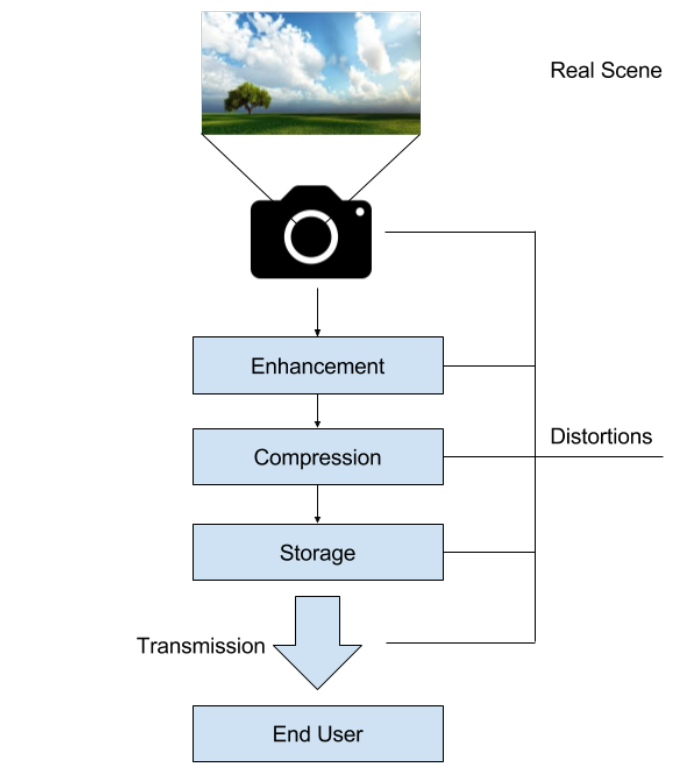
\includegraphics[width=\linewidth]{figures/digitalsteps.png}
  \caption{Digital images suffer from distortions on every step.}
  \label{fig:digimgs}  
\end{figure}
  
End users tend to be more inclined to select a content provider, a service provider, and a display device that can better meet their image quality expectations at delivery. Thus, optimizing these respective technologies to deliver perceptually good results becomes crucial for all content providers, service providers, and display providers, and in order to do so, perceptual image quality needs to be estimated. In addition, in order to determine the perceptual quality, this estimation process should be automated as much as possible to make it independent of the availability of human observers. 

Image Quality Assessment (IQA) aims to measure the perceived quality of the visual signal based on its statistical characteristics and human perceptual mechanism, which is widely required in numerous applications for image processing. IQA plays a vital role in guiding, implementing, optimizing and verifying many visual processing algorithms and systems \cite{Lin2011,Wang2018,Wang2018a,Zhang2016}. 
In particular, image compression is one of IQA's most representative applications, which can be used in the process of optimizing rate distortion to obtain compressed images with better visual quality at the same bit-rate level.  \cite{Channappayya2008,Chen2010,Wang2012,Zhang2017,Zhang2017a,Ma2016}. 
The traditional methods of image compression mainly use the quality metrics based on signal-fidelity, which are less correlated with human perceptual quality , e.g., MAE (mean absolute error), MSE
(mean square error), SNR (signal-to-noise ratio), PSNR (peak
SNR) and their relatives. 
While these metrics have many favorable properties, e.g. clear physical meaning and high calculation efficiency, they severely impede the improvement in compression performance by further reducing image visual redundancies due to their poor consistency with human visual perception. 

Many perceptual quality metrics have been proposed over the past few years to obtain more consistent measures with human visual perception. 
According to the availability of a reference image, these methods can be divided into three categories, i.e., full reference (FR) ones where the pristine
reference image is available, reduced reference (RR) ones
where partial information of the reference image is available
and no reference (NR) ones where the reference image is
unavailable. 
For image compression problem, the reference images are available at the encoder side such that the FR-IQA
algorithms are applicable.

Many FR-IQA based algorithms have been proposed over time. One class of these
algorithms including SSIM \cite{Wang2012}, FSIM \cite{Zhang2011}, RFSIM \cite{Zhang2010} use handcrafted features (attributes (edge, color, etc.) in data (images) that are relevant to the
modeling problem) that supposedly captures relevant factors affecting image quality. 
Although their performance is acceptable, there is still large room for improvement regarding the accuracy with which they reproduce human judgment of quality. 
Another set of algorithms, including convolutional neural network
(CNN) based approaches \cite{Bosse2018,Kang2015}, employ automatic learning of features from the
raw image pixels, which are superior and more efficient as they make feature selection automatic and embedded within the system itself.

\section{Motivation}

Most of the existing IQA
databases usually contain limited distortion levels (5-6 levels)
covering the whole quality range from \enquote{Bad} to \enquote{Excellent},
which make the images in adjacent distortion levels obviously
different and easy to rank. 
To describe the obvious and subtle quality differences between two images, Zhang \textit{et al} \cite{Zhang2019} use
the terms \enquote{coarse-grained} and \enquote{fine-grained}.
More specifically, the images with \enquote{coarse-grained} quality differences correspond to the compressed ones generated using the same codec at obvious different bitrates, while the images with \enquote{fine-grained} quality difference correspond to the compressed ones generated using
different optimization methods at the same bitrate. 
Therefore, these databases with coarse-grained distortion variations
for the same image may not be able to provide sufficient
information to further improve the performance of IQA algorithms in evaluating fine-grained quality differences. 

Another weakness for the existing IQA databases is that
they only contain a few reference images with limited visual content. 
To solve this problem patch-based methods are gradually used in IQA, e.g. CNN-IQA \cite{Kang2014}, CORNIA \cite{Ye2012}
The patch-based learning methods requires the \enquote*{ground truth} of patch quality for training
but there are only the ground truth quality of images instead
of patches in IQA datasets.
To deal with this problem, existing works usually assign the image quality score to all patches
in this image as their \enquote*{ground truth}, e.g. CNN-IQA \cite{Kang2014}. 
This approach might introduce much noise in patches labels because in some distortion types the quality of patches in one
image varies much and the patches quality score can’t be
simply assigned as the image quality core. 

Based on all these observations, this project promotes IQA in the new challenges of fine-grained quality assessment task by constructing a large-scale Image-Patch Quality Assessment database with fine-grained distortion differences. 
We also analyze 7 state-of-the-art IQA algorithms on the proposed database and show that there is still a large room to improve the IQA in the prediction of the fine-grained quality preference. 
Finally, we propose an FR Image-Patch model to help estimate the \enquote*{ground truth} quality of patches based on a state-of-the-art CNN architecture.   
   
\begin{figure}[H]
  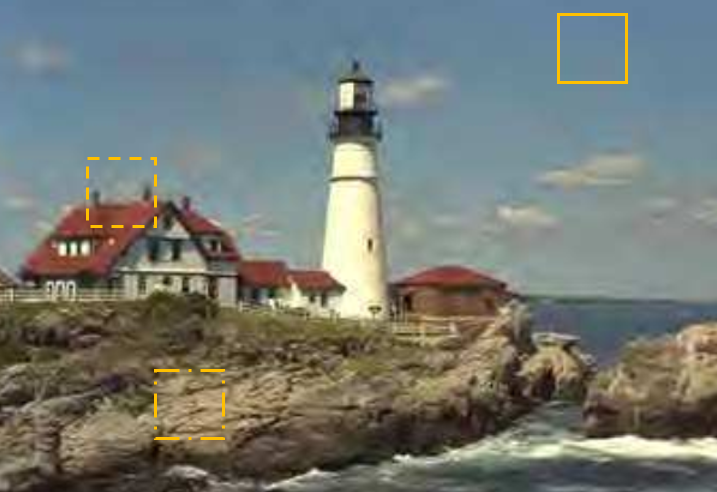
\includegraphics[width=\linewidth]{figures/first.png}
  \caption{Example of JPEG distorted image. Different patches have different qualities.}
  \label{fig:dist-exmaple}
\end{figure}


\section{Contributions}

This thesis provides the following contributions:

1. \textbf{Image-Patch Quality Assessment dataset}

To our knowledge, this dataset is the first one constructing to provide benchmark for compressed image patch quality assessment, and also benefit for perceptual-based image compression. 
The existing databases with coarse-grained quality are inefficient to evaluate IQA algorithms especially patch-based methods on images with fine-grained quality differences. 
In perceptual-based image compression problem, for each coding block there are many coding modes to select a according their rate-distortion costs. Therefore, the proposed dataset can help researchers in image compression community to select the best IQA method to do the perceptual based image optimization. 7 well-know IQA algorithms are evaluated and analyzed on the proposed database to reveal some limitations of the existing algorithms.

2. \textbf{Deep Image-Patch Neural Network Design}

We also investigate different FR methods to model the relationship between the image patch and patch quality score. 
After multiple of experiments, Deep Image-Patch Quality Assessment (DIPQA) is proposed to address the problem in and end-to-end optimization. 
We adapt the concept of Siamese networks know from classification task \cite{BROMLEY2004,Chopra2005} that allow for a join regression of the features extracted from the reference and distorted patch using a deep convolution neural network. 

\section{Thesis Outline}

The rest of this thesis is organized as follows. After this introduction, we present the literature review in Chapter 2 in which we introduce the fields of image quality assessment and deep learning. Next, our methodology is described in Chapter 3. Chapter 4 shows the evaluation of our database and proposed neural network based on experiment result. Finally, the conclusions and future directions are given in Chapter 5.